\documentclass[10pt,a4paper,twoside]{article}

\usepackage{graphicx}
\usepackage{amsmath}
\usepackage{multicol}
\usepackage{amssymb}
\usepackage{tabularx}
\usepackage{xcolor}
\usepackage{fontspec}
\usepackage{titlesec, blindtext}
\usepackage[spanish,es-tabla]{babel}
\usepackage{tocloft}
\usepackage[
    hyperindex=true,
    bookmarks=true,
    bookmarksnumbered=true,
    hidelinks,
]{hyperref}
\usepackage[all]{hypcap}
\usepackage[labelfont=bf]{caption}
\usepackage{float}
\usepackage{bytefield}
\usepackage{listings}
\usepackage[
    top=2cm,
    inner=2cm,
    outer=1.5cm,
    bottom=2.5cm,
]{geometry}
\usepackage[skip=5pt]{parskip}

\setmainfont[Ligature=TeX]{Times New Roman}
\setlength\columnsep{0.5cm}
\setlength{\parindent}{0in}
\makeatletter
\renewcommand{\fnum@figure}{Fig. \thefigure}
\makeatother
\captionsetup{labelsep=period}
\titleformat{\section}[block]{\centering\large\bfseries}{\thesection. }{0.1em}{}
\titlespacing{\section}{0em}{0.3em}{0.3em}
\pagenumbering{gobble}

\bibliographystyle{unsrt}

\begin{document}

\begin{center}
    \bfseries\fontsize{22pt}{27pt}\selectfont\par
    Desarrollo de una herramienta de análisis de tráfico de red y su uso en algoritmos de ML para la detección de ataques.
    \par
\end{center}

\bigskip

\begin{center}
    \large\par
    Raul Rabadan Arroyo
    \par
\end{center}

\begin{center}
    \par
    Estudiante en Grado de Ingeniería Informática de la EPSEVG-UPC
    \par
\end{center}

\smallskip

\begin{multicols*}{2}
    \section*{Resumen}

    En este Trabajo de Final de Grado (TFG) se hace el desarrollo de PacketPincer, una herramienta de análisis de red, y se demuestra su funcionamiento a partir de analizar trazas de tráfico de red y el uso de los datos resultantes para entrenar modelos con Machine Learning. La herramienta desarrollada puede ser utilizada como componente en sistemas  de detección de intrusiones y tiene el potencial para ser extendida con más funcionalidades en el futuro. Se ha hecho uso de Rust para el desarrollo de la herramienta y es capaz de generar 72 características continuas, 2 discretas para el protocolo de transporte y una identificación de cada flujo compuesta por 7 valores. Adicionalmente, hay soporte para el etiquetado automático a partir de un fichero CSV. Con los registros generados por la herramienta, se ha entrenado un modelo supervisado de Machine Learning (ML) para detectar flujos de red malignos, logrando una puntuación F1 media del 98.66\%.

    \section{Introducción}
    
    La ciberseguridad es una de las fronteras del conocimiento que ha tomado más relevancia estos últimos años. Se aplican numerosas y diversas técnicas en conjunto para mantener la disponibilidad, integridad y confidencialidad de la información, esté esta almacenada como en tránsito. Estas técnicas van desde medidas criptográficas para proteger la información, hasta el análisis del tráfico de red para detectar y poder bloquear comportamientos maliciosos.

    En muchos casos, los tráficos de red maliciosos son identificados cuando estos ya han ocurrido o están generando problemas activamente para el resto de usuarios de la red. La gran utilidad que supondría la detección de ataques en su inicio o incluso antes de que ocurriesen es una meta en la que me gustaría colaborar. Llegar a este ideal es altamente difícil. Sin embargo, tenerlo como horizonte para dirigir el camino y acercarse lo máximo posible a este, ofrece la capacidad de mejorar la mitigación contra posibles adversarios.
    
    La motivación para la realización de este Trabajo Final de Grado (TFG) surge de mi participación, a través de una beca de colaboración, con el grupo de investigación Centre de Recerca d’Arquitectures Avançades de Xarxes (CRAAX) y mi interés por la aplicabilidad de los sistemas de ML en entornos limitados, como dispositivos IoT, así como en entornos reales donde los tiempos de respuesta deben ser imperceptibles. Durante la colaboración, he utilizado herramientas de extracción de características para la caracterización de flujos de red. Sin embargo, estas presentaban ciertas limitaciones e inconvenientes, los cuales me han impulsado a querer desarrollar una alternativa.

    El resto del artículo está estructurado de la siguiente manera. Primero, veremos en la Sección \ref{cicflowmeter} la herramienta que ha servido de principal inspiración para el desarrollo del trabajo y se comentarán sus potenciales mejoras. A continuación, en la Sección \ref{funcherramienta}, se indicará la estructura general de la herramienta, qué librerías se han utilizado y modificaciones necesarias a una de estas. Después de esto, se mostrará dentro de las secciones \ref{casoexec} y \ref{casoml} una aplicación en un caso de ML para mostrar su utilizad. Finalmente, terminaremos con las conclusiones y el trabajo futuro en Sección \ref{tabajofuturo} y Sección \ref{agradecimientos}, respectivamente.

    \section{CICFlowMeter} \label{cicflowmeter}

    CICFlowMeter es una herramienta para generar y analizar flujos de red creada por el Canadian Institute for Cybersecurity \cite{cicflowpost} \cite{icissp17} \cite{cicflowrepo}. Permite obtener información acerca de flujos bidireccionales sobre IP a partir de trazas de red en archivos con el formato PCAP. Adicionalmente, los protocolos de transporte que soporta son UDP y TCP. Por cada flujo, genera siete columnas identificativas y añade 76 características continuas. De estas características generadas, hay algunas como 'Fwd Packet Length Mean' y 'Fwd Segment Size Avg' que parecen estar representando el mismo valor.

    La herramienta soporta exclusivamente trazas y la captura de paquetes que provengan de la capa de enlace Ethernet. No ofrece soporte para Linux Cooked Capture (SLL), el cual es utilizado en contextos en los cuales se capturan datos de varias interfaces de red simultáneamente o se quiere descartar información de la capa de Ethernet. Adicionalmente, no parece tener soporte para la desfragmentación de paquetes IP.

    En el momento de utilizar la herramienta, se observó que se introducían cabeceras duplicadas en los archivos CSV. Esto era causado debido a que el módulo cic.cs.unb.ca.jnetpcap.FlowGenerator, en la función dumpLabeledFlowBasedFeatures, escribía la cabecera dos veces, una después de generar el archivo y otra después de escribir todos los flujos completos. No fue posible encontrar una indicación de por qué se realizaba de esta manera, por tanto, se puede asumir que se trató de un error.

    Durante el análisis del código, se han identificado bloques de código comentados (puestos en forma de comentario para que sean ignorados en el momento de ejecución) además de tabulación inconsistente. Es posible que la causa de esto haya sido que el código ofrecido en el repositorio de GitHub esté desactualizado o se haya decidido no continuar el trabajo en CICFlowMeter.

    Por estas razones, se ha considerado que el desarrollo de otra herramienta que haga una tarea equivalente sin estos inconvenientes podría ser una aportación útil.

    \section{Estructura de la herramienta} \label{funcherramienta}

    PacketPincer se ha desarrollado haciendo uso de Rust. Se ha escogido este lenguaje para el desarrollo de la herramienta debido a su capacidad para escribir código de bajo nivel, su alto rendimiento, su énfasis en el código correcto, la calidad de las herramientas asociadas y el gran número de librerías disponibles. El nombre ha sido escogido por el análisis que realiza de los paquetes y por intentar seguir el estilo de nombres de los programas hechos en Rust.

    El ciclo principal del programa tiene diversas fases. Primero, se accede cada paquete de forma secuencial. Para cada uno de estos se trata de reensamblarlo, si es un paquete IP fragmentado, y luego decodificarlo. Si esto se realiza con éxito, se extrae su identificador y se determina si pertenece a un flujo conocido o a uno nuevo, actualizando el estado interno en consecuencia. Finalmente, se comprueba si hay flujos de red que han pasado más de cierto tiempo sin actividad. En caso afirmativo, se emiten las estadísticas acumuladas y se descarta la información de esos flujos.

    El programa está principalmente ideado para ser ejecutado por terminal. Esto implica que es necesario desarrollar la capacidad de permitir especificar qué argumentos deben ser proporcionados al programa en el momento de ejecutarlo desde la terminal. Además, se ha implementado soporte para que el programa sea capaz de responder a las señales que pueda recibir durante su ejecución. Para facilitar esta tarea, hemos hecho uso de dos librerías. La primera librería utilizada es \texttt{clap} \cite{Knapp_clap_2024} para definir los parámetros por consola. Estos permiten al usuario seleccionar si emitir resultados a archivos o a la salida estándar, proporcionar un archivo 'ground truth' para etiquetar los datos y si hacer un análisis de trazas de red o capturar tráfico activamente. La segunda librería es \texttt{ctrlc} \cite{controlc}, la cual nos permite detectar de forma sencilla que se ha enviado una interrupción al programa. En caso de recibirla, se emiten todos los resultados y se finaliza la ejecución.

    Como ya vimos, el ciclo principal se inicia con la lectura de paquetes. Para realizar esto, hemos hecho uso de la librería \texttt{pcap} \cite{rustpcap}, la cual nos permite obtener datos desde una traza de paquetes o una interficie de red. Sin embargo, no tiene soporte para trabajar a partir de una colección de trazas. Debido a que necesitábamos realizar esto, se ha desarrollado una capa adicional alrededor de las funcionalidades proporcionadas por la librería para poder leer de un conjunto de archivos, los cuales pueden tener solapamientos temporales entre ellos. Este proceso no ha sido trivial debido a la gestión de la memoria y las restricciones impuestas por el lenguaje. El principal problema ha sido que los paquetes que la librería \texttt{pcap} nos daba acceso contenían referencias 'prestadas' a memoria y relacionadas con el mecanismo de leer más paquetes. Esto provocaba que, si intentábamos dar al usuario acceso directo a los paquetes y a continuación actualizar el estado interno de la lectura, el compilador no podía garantizar un uso correcto de la memoria. Para solucionar esto, se ha hecho uso de una clausura. Esta permite que el usuario de la capa indique la función que quiere ejecutar para hacer el análisis, mientras que nuestro módulo indica explícitamente las restricciones de uso. De esta manera, el compilador ha podido verificar el uso correcto de la memoria y se ha ofrecido la funcionalidad que se deseaba.

    Una vez obtenido los paquetes, se ha de realizar el paso de descodificación. Para esta tarea, se ha empleado la librería \texttt{etherparse} \cite{etherparse}. Esta librería originalmente tenía soporte para interpretar, entre otros, tramas Ethernet, paquetes IP, datagramas UDP y segmentos TCP. Sin embargo, no ofrecía soporte para interpretar SLL, el cual era uno de los formatos con los que queríamos trabajar. Debido a que la librería tenía soporte para la mayoría de puntos necesarios, además de  ofrecer una interfaz sencilla, se decidió hacer una extensión de esta para añadirle soporte de SLL. Después de trabajar durante una semana, se añadieron 4145 líneas de código y se eliminaron 141. Estas incluyen toda la lógica para interpretar el formato, tests y documentación asociada. El 29 de abril se ofreció al desarrollador original la combinación de las mejoras a través de un 'pull request' \cite{slladdsllpr} en el repositorio original. Después de unas revisiones, los cambios fueron integrados a la rama principal del proyecto.

    La extracción del identificador de la comunicación es sencilla. Se acceden a las cabeceras de red y de transporte para obtener las direcciones de IP de origen y la de destino, el protocolo de transporte utilizado y los puertos de origen y de destino. Una vez obtenido, este se compara con los flujos activos conocidos y se determina si es un flujo nuevo o forma parte de los ya existentes. A continuación, se acumula información estadística para poder emitir un resultado en el momento en que el flujo deje de considerarse activo.

    % Indicar defragmentación?

    La información que se acumula durante el transcurso de la ejecución es diversa. Las estadísticas escogidas para generar han sido basadas en las utilizadas en CICFlowMeter. La información acumulada durante la ejecución consiste en:

    \begin{itemize}
        \item Marca de tiempo del primer y último paquete.
        \item Si se ha detectado el protocolo de transporte UDP o el TCP.
        \item Recuento de paquetes diferenciado por dirección.
        \item \texttt{RunningStat} para el número de bytes enviado, diferenciado y sin diferenciar por dirección.
        \item \texttt{RunningStat} para el periodo de llegada entre paquetes diferenciados por dirección.
        \item Información sobre los flags TCP observados por dirección.
        \item \texttt{RunningStat} para la información específica sobre las longitudes de cabeceras y datos en la capa de transporte.
        \item El número de paquetes vacíos hacia el receptor inicial.
        \item \texttt{RunningStat} para mantener información sobre los tiempos de actividad.
    \end{itemize}

    Los \texttt{RunningStat} mencionados son una estructura que se ha programado para calcular incrementalmente valores estadísticos. Nos permite obtener en cualquier momento el número de valores acumulados, la suma, el mínimo, el máximo, la media y la desviación estándar. Para calcular las dos últimas, mantenemos valores parciales de la manera que se indica en la página 232 de 'The art of computer programming' \cite{10.5555/270146}. Específicamente, primero se define la recurrencia \ref{eq:meanrec} para calcular la media de forma iterativa. A continuación, se utiliza esta para obtener la recurrencia de la 'diferencia al cuadrado' mostrada en \ref{eq:sqrrec}, de la cual podemos obtener la varianza como se indica en \ref{eq:variancereq}. A partir de esta, podemos obtener la desviación estándar (\sigma).

    \begin{equation} \label{eq:meanrec}
        \biggl\{
            \begin{array}{l}
              M_{0} = 0\\
              M_{k} = M_{k-1} + {\frac{ x_{k} - M_{k-1} }{k}}  \\
            \end{array} 
    \end{equation}
    
    \begin{equation} \label{eq:sqrrec}
    \biggl\{
        \begin{array}{l}
            S_{0} = 0 \\
            S_{k} = S_{k-1} + ( x_{k} - M_{k-1} ) * ( x_{k} - M_{k} )
        \end{array}      
    \end{equation}
    
    \begin{equation} \label{eq:variancereq}
    \biggl\{
        \sigma^2_{k} = {\frac{S_{k}}{(k - 1)}}
    \end{equation}

    Finalmente, una vez se considera un flujo cerrado, se etiqueta si es posible y se emite el resultado. El etiquetado se realiza a partir de un fichero 'ground truth' proporcionado por el usuario, el cual ha de incluir un par de direcciones IP, el protocolo de transporte utilizado, la marca de tiempo de inicio y final expresadas en tiempo UNIX y la etiqueta deseada. Se trata de encontrar la mejor coincidencia en este con el flujo cerrado y, en caso de no encontrar nada, se asigna la etiqueta 'unknown'. Una vez realizado esto, se emite el resultado según cómo lo haya indicado el usuario. La primera opción es emitirlo a la salida estándar, la cual puede estar conectada a la consola, a un archivo o a una 'pipe' que pasa los resultados a otro programa. La segunda, es escribirlo en archivos CSV con un prefijo indicado por el usuario. Para evitar generar archivos intratables, cada 10 millones de linias se empiezan a escribir en un archivo CSV nuevo.

    \section{Aplicación de la herramienta} \label{casoexec}

    Para mostrar un posible uso de la herramienta, hemos utilizado tres conjuntos de datos etiquetados, de los cuales se nos ofrecen las trazas de red originales. De estos, hemos extraído y simplificado las etiquetas disponibles y a continuación ejecutado la herramienta sobre las trazas.

    El primer conjunto de datos utilizado ha sido CIC-DDos\-2019 \cite{8888419}. Este ha sido creado por el Canadian Institute for Cybersecurity que contiene trazas de dos días en los que aparece tráfico benigno y serie de ataques DDoS típicos. Para extraer las etiquetas, primero hemos leído los campos conteniendo las direcciones IP, protocolo, marca temporal de inicio, duración del flujo y etiqueta. A continuación, las marcas temporales se han ajustado para que estén expresadas en tiempo UNIX. Después de esto, se ha convertido la columna de duración en la marca temporal de finalización. Finalmente, se han eliminado los registros con protocolos inválidos, expresado y puesto el nombre de las columnas y etiquetas al formato que la herramienta esperaba.
    
    El segundo conjunto consiste en BoT-IoT \cite{DBLP:journals/corr/abs-1811-00701}. Este ha sido creado por la University of New South Wales Canberra, Australia y para generarlo, se desarrolló un entorno de red realista, consistiendo en plataformas de red, dispositivos IoT simulados y extracción de características y análisis forense. Para la extracción de las etiquetas, hemos hecho un proceso similar a lo anterior. Sin embargo, en vez de duración, tenemos directamente el tiempo del último paquete y la etiqueta está separada en una categoría y una subcategoría. Para mantener consistencia, hemos juntado las dos últimas para representar una única etiqueta. Adicionalmente, ha sido necesario convertir todos los protocolos de transporte a su representación numérica y eliminar los registros con protocolos inválidos.
    
    El tercero ha sido TON-IoT \cite{MOUSTAFA2021102994}. Este ha sido creado por la University of New South Wales Canberra, Australia y para generarlo se estructuró un entorno de red con tres capas llamadas Edge, Fog y Cloud para simular un entorno realista. Para la extracción de las etiquetas, hemos hecho un proceso similar al primer dataset. La diferencia ha sido que la marca temporal estaba representada como tiempo UNIX, pero en formato decimal. Es decir, con una parte entera con los segundos y una parte decimal con la fracción de segundo. También ha sido necesario representar los protocolos en formato numérico y descartar los registros con protocolos inválidos.

    Una vez extraídas las etiquetas, se procedió a ejecutar la herramienta sobre los diferentes conjuntos de datos. Podemos ver en la Tabla \ref{table:statsevalpacketoffline} cómo la mayoría de paquetes de BoT-IoT fueron procesados correctamente, mientras que parte de los paquetes de los otros no se pudieron tener en cuenta para la generación de estadísticas. En la Tabla \ref{table:statstimeoffline} podemos observar cómo la herramienta ha podido tratar en un tiempo razonable los paquetes que estaban repartidos por horas o incluso días. Finalmente, en la Tabla \ref{table:generatedfilesoffline} podemos observar la magnitud de los datos resultantes de la ejecución.

    \begin{table}[H]
        \begin{center}
            \resizebox{\columnwidth}{!}{%
                \begin{tabular}{|c | c c c |} 
                    \hline
                    & \textbf{CIC-DDoS2019} & \textbf{BoT-IoT} & \textbf{TON-IoT} \\
                    \hline
                    Paquetes procesados & 312 191 170 & 549 787 584 & 213 236 852 \\
                    Paquetes válidos    & 286 881 800 & 549 057 279 & 175 845 321 \\
                    \hline
                \end{tabular}
            }
        \end{center}
        \caption{Paquetes procesados y válidos en el análisis}
        \label{table:statsevalpacketoffline}
    \end{table}

    \begin{table}[H]
        \begin{center}
            \resizebox{\columnwidth}{!}{%
                \begin{tabular}{|c | c c c |} 
                    \hline
                    & \textbf{CIC-DDoS2019} & \textbf{BoT-IoT} & \textbf{TON-IoT} \\
                    \hline
                    Tiempo total   & 7m 17,665s & 7m 31,202s & 3m 32,303s \\
                    Tiempo usuario & 5m 50,915s & 7m  0,735s & 3m  4,560s \\
                    Tiempo kernel  & 1m 50,915s & 0m 28,419s & 0m 26,181s \\
                    \hline
                \end{tabular}
            }
        \end{center}
        \caption{Tiempos de análisis}
        \label{table:statstimeoffline}
    \end{table}

    \begin{table}[H]
        \begin{center}
            \resizebox{\columnwidth}{!}{%
                \begin{tabular}{|c | c c c |} 
                    \hline
                    & \textbf{CIC-DDoS2019} & \textbf{BoT-IoT} & \textbf{TON-IoT} \\
                    \hline
                    Número de archivos &          5 &          1 &          3  \\
                    Flujos totales     & 48 385 896 &  6 077 653 & 27 005 789  \\
                    Bytes totales      &    29 GiB  & 3,8 GiB    & 16 GiB      \\
                    \hline
                \end{tabular}
            }
        \end{center}
        \caption{Archivos generados durante el análisis}
        \label{table:generatedfilesoffline}
    \end{table}

    Debido a la estructura de los datos originales, los flujos etiquetados como benignos son solo un 0,846 \%. Adicionalmente, tenemos que las etiquetas de ataques tienen niveles de especificidad distinta y están concentradas en diversas variaciones de ataques de DoS.

    \section{Uso de los datos generados} \label{casoml}

    Para mostrar un ejemplo sencillo del uso de los datos generados, se ha decidido hacer un modelo de detección de flujos de tráfico regular y tráfico de ataque. Ha sido necesario realizar un muestreo para poder tratar los datos con la capacidad de cómputo disponible. 

    Para realizar el preprocesamiento inicial, se ha tomado cada archivo CSV generado y se han remplazado las etiquetas específicas de ataques por 'malign', manteniendo las etiquetas de tráfico normal como 'benign'. A continuación, se ha realizado un muestreo estratificado del 0.5\% de los datos, reduciendo los aproximadamente 80 millones de registros a 358 778. Una vez realizado el muestreo, se ha aplicado el logaritmo a las características continúas, habiéndoles sumado 1 para evitar generar valores infinitos. Después de esto, se ha realizado un escalado de todos los datos para que estén localizados en el rango $[0, 1]$. 
    
    Debido a que tenemos una cantidad de características no reducida, hemos ejecutado una implementación del algoritmo Boruta \cite{borutapy} para realizar una selección de características más representativas. Al ejecutarlo, nos ha descartado las características del recuento de paquetes con los flags CWR, ECC y URG en las cabeceras TCP. Esto es esperable, ya que la extensa mayoría de estas eran 0.

    Con los datos preparados, se ha hecho un split 70/20/10 para entrenar los modelos, seleccionar el que tenga mejor rendimiento y comprobar la capacidad de generalización del modelo seleccionado con datos que aún no ha visto. 

    El rendimiento de los modelos al entrenarlos con el 70\% y validarlos con el 20\% se puede observar en la Tabla \ref{table:rendimientomodelos}. Podemos ver cómo, en general, el rendimiento es muy bueno. El modelo que parece tener mejor rendimiento es el que se basa en bosques aleatorios, el cual entrena una serie de árboles de decisión con técnicas adicionales para mejorar la precisión mientras se evita el sobreajuste \cite{sklearnrandomforest}.

    \begin{table}[H]
        \begin{center}
            \resizebox{\columnwidth}{!}{%
                \begin{tabular}{|c | c c c |} 
                    \hline
                    \textbf{Modelo} & \textbf{Exactitud} & \textbf{F1 macro}  & \textbf{F1 avg} \\
                    \hline
                    Naive bayes        & 0.710405          &         0.440790  &          0.822148 \\
                    Arbol de decisión  & 0.999546          &         0.987305  &          0.999548 \\
                    KNN                & 0.998704          &         0.963123  &          0.998699 \\
                    Red neuronal       & 0.997771          &         0.941093  &          0.997843 \\
                    Votación           & 0.999183          &         0.977438  &          0.999192 \\
                    Bagging            & 0.999663          &         0.990481  &          0.999663 \\
                    AdaBoost           & 0.999093          &         0.974074  &          0.999087 \\
                    Bosques aleatorios & \textbf{0.999689} & \textbf{0.991213} & \textbf{0.999689} \\
                    \hline
                \end{tabular}
            }
        \end{center}
        \caption{Rendimiento de modelos sobre los datos de entrenamiento y selección}
        \label{table:rendimientomodelos}
    \end{table}

    Para comprobar si el mejor modelo es capaz de generalizar a más datos, se ha tomado el 90\% de datos utilizados para entrenar y validar y entrenaremos un nuevo modelo. Con este, generaremos nuevas estadísticas con el 10\% restante de comprobación y verificaremos si se mantiene su rendimiento.

    \begin{table}[H]
        \begin{center}
            \begin{tabular}{|c | c c c |} 
                \hline
                & \textbf{Precisión} & \textbf{Recuperación} & \textbf{F1}\\
                \hline
                benign               & 0.988024 & 0.959302 & 0.973451 \\
                malign               & 0.999634 & 0.999895 & 0.999765  \\
                \hline
                exactitud            &          &          & 0.999533 \\
                F1 macro             & 0.993829 & 0.979599 & 0.986608 \\
                F1 avg               & 0.999530 & 0.999533 & 0.999530 \\
                \hline
            \end{tabular}
        \end{center}
        \caption{Resultados de clasificación del modelo final sobre los datos de test}
        \label{table:selectedresults}
    \end{table}
    
    \begin{figure}[H]
        \begin{center}
            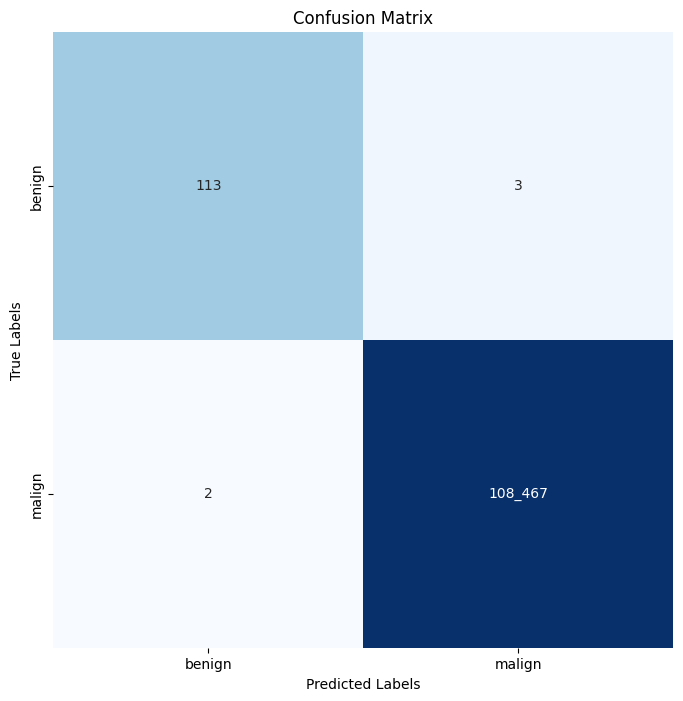
\includegraphics[width=\linewidth]{../report/media/packet_pincer_train_model_random_forest_selected.png}
        \end{center}
        \caption{Matriz de confusión del modelo final sobre los datos de test}\label{fig:selectedmatrix}
    \end{figure}
    
    El entrenamiento final ha tardado 5.8 segundos y la predicción 2.2 centésimas de segundo. Se podría considerar que el modelo es relativamente rápido y si las condiciones fuesen iguales podría procesar unos 1.7 millones de paquetes por segundo. Las puntuaciones F1 y la exactitud han mejorado ligeramente comparado con la selección de modelos como podemos ver en la Tabla \ref{table:selectedresults}. Si miramos la matriz de confusión de la Figura \ref{fig:selectedmatrix}, podemos ver como solo se han clasificado incorrectamente 3 flujos malignos como benignos y 10 flujos benignos como malignos.

    Con esto, podemos afirmar que el modelo seleccionado puede generalizar a datos nuevos, siempre que sigan la distribución y el formato de los datos con los que hemos trabajado. Es posible que en un entorno distinto el rendimiento del modelo no se mantenga.
    
    \section{Conclusiones} \label{conclusiones}

    Durante el transcurso del proyecto, hemos analizado diferentes conjuntos de datos y herramientas disponibles. En este proceso, notamos la falta de una herramienta que ofreciera el etiquetado automático de flujos con características similares a CICFlowMeter. Es decir, el poder generar estadísticas de flujos con etiquetas asociadas tanto en tiempo real como con trazas de red para entrenar modelos directamente de estas. Una vez desarrollada, el despliegue de esta herramienta no requiere de una gran complejidad, ya que es un programa compilado el cual requiere una cantidad limitada de librerías dinámicas.

    Cuando se utilizó la herramienta para entrenar modelos, se pudo observar que la mayoría de modelos entrenados muestran un buen rendimiento, indicando que los datos generados por la herramienta permiten caracterizar el comportamiento de los flujos. Sin embargo, los resultados específicos obtenidos con los modelos generados tienen el potencial riesgo que solo funcionen correctamente sobre los entornos sintéticos originales donde se generaron los datos y que en una situación real los resultados varíen.
    
    \section{Trabajo futuro} \label{tabajofuturo}

    Existen muchas posibles ramas de trabajo futuras como continuación de este proyecto. Por cada parte de la herramienta, es posible añadir nuevas características. Adicionalmente, se puede tratar de integrar en entornos más generales y hacer uso de esta bajo otros contextos.

    La herramienta solo tiene soporte para dos capas de enlace y dos protocolos de transporte. Se podría añadir soporte para analizar flujos de comunicación en diferentes capas de la pila OSI y más cantidad de protocolos aceptados. Ejemplos pueden ser comunicaciones transmitidas sobre Bluetooth o 5G e incluso analizar si las peticiones de la capa de aplicación son válidas. Otra opción es añadir soporte para correlacionar diferentes flujos, sea para mejorar la detección de ataques DDoS o incluir información sobre comunicaciones que se transmitan en flujos paralelos como en RTP/RSTP.

    Adicionalmente, hay partes de la herramienta donde se hacen copias de los datos o no se limita la capacidad máxima de las estructuras de datos. No se ha tenido en cuenta este punto en el desarrollo para poder tener un código más simple. Sin embargo, si se llegase a desplegar una herramienta y un atacante tratase de, por ejemplo, tomar ventaja de cómo reconstruimos paquetes IP fragmentados, sería posible provocar que se termine la memoria RAM disponible. Una posible solución simple para evitar esto es descartar cualquier paquete fragmentado y no tratar de reconstruirlo. 

    Otro punto de posible mejora consiste en la creación de mayores tests del código para asegurar su buen funcionamiento incluso en casos inesperados. Con herramientas de cobertura de código se podrían detectar flujos de ejecución, los cuales no tienen tests asociados y podrían tener errores lógicos ocultos.

    Otra categoría de posible trabajo futuro consiste en aplicar la herramienta sobre otros algoritmos de ML o conjuntos de datos. Observar si los modelos son capaces de generalizar a otros entornos puede indicar con mayor certeza si la herramienta puede ser utilizada en cualquier tipo de contexto o si es más efectiva en zonas específicas de la infraestructura.

    \section{Agradecimientos} \label{agradecimientos}

    Primero de todo, quiero agradecer a mis padres por el apoyo y palabras de aliento que he recibido durante el transcurso de mis estudios y de esta fase final del grado. Sin este, no hubiese sido posible haber llegado hasta este punto ni haber tenido la capacidad o la perseverancia para el desarrollo del trabajo.

    A continuación, agradezco al profesorado, el cual me ha permitido descubrir y consolidar conceptos que de otra manera hubiese sido mucho más difícil obtener. Con especialidad a Ester Simo, la directora del proyecto, que ha ayudado a tener un control del progreso del proyecto, la detección de mejoras en la redacción y el desbloqueo para saber por dónde continuar en los momentos en que los resultados obtenidos eran muy inferiores a lo esperado.

    Finalmente, quiero mostrar mis agradecimientos a la Escola Politécnica Superior d'Enginyeria de Vilanova i la Geltrú y al Centre de Recerca d'Arquitectures Avançades de Xarxes (CRAAX), por ofrecerme la oportunidad de realizar mis estudios, prácticas y Trabajo Final de Grado con ellos.

    \bibliography{refs}

\end{multicols*}
\end{document}
